\section{Avoiding Spurious Correlation: Using Inclusion Maps}

\subsection{The Problem of Timing: When Did What Happen?}

\vspace{0.5em}
In high-frequency trading, the difference between acting on a signal and reacting to one can come down to microseconds. But in a globally distributed system with machines operating asynchronously, that’s not an easy distinction to make. Two events might appear causally related simply because one is observed before the other. However, was it truly earlier, or just received sooner due to network latency?

This creates a fundamental challenge: \textbf{how can we determine whether one trade caused a market reaction, or merely appeared to?}

To answer that, we need more than statistical correlation. We need a structure that captures the \textbf{temporal flow of information}: one that respects both event order and system delays.

That’s where vector clocks come in.


\begin{figure}[H]
\centering
\begin{tikzpicture}[every node/.style={font=\footnotesize}]

% Panel 1 — Trader 1 thinks they caused a reaction
\comicpanel{0}{4}
  {Trader A}
  {Trader B}
  {That price spike right after my trade? You're welcome.}
  {(0,-0.6)}

% Panel 2 — Trader B is skeptical
\comicpanel{6.5}{4}
  {Trader A}
  {Trader B}
  {Pretty sure the spike hit our system before your trade even left the building.}
  {(0,-0.5)}

% Panel 3 — Trader A confused
\comicpanel{0}{0}
  {Trader A}
  {Trader B}
  {But... my logs say I traded first. Time is real, right?}
  {(0,0.5)}

% Panel 4 — Trader B drops the clock truth
\comicpanel{6.5}{0}
  {Trader A}
  {Trader B}
  {In distributed systems, time is just a polite suggestion. Use vector clocks.}
  {(0,0.6)}

\end{tikzpicture}
\caption{In high-frequency trading, causality is a microsecond mirage — unless you bring a vector clock.}
\end{figure}



\subsection{Vector Clocks: Capturing Temporal Causality in Trading}

\vspace{0.5em}
\noindent
Imagine a group of traders chatting in a messaging app, but everyone is on slightly different Wi-Fi. Each time a message (or trade) is sent, it’s timestamped locally. Now suppose one trader tries to argue that their message caused a market reaction; but another trader can show, based on message arrival times, that their system had already reacted before the first message even appeared. Clearly, the timeline doesn’t add up.

This kind of ambiguity is common in high-frequency trading, where machines operate asynchronously and respond to signals within microseconds. Determining what actually caused a price movement — and what merely reacted to one — becomes a serious challenge.

\textbf{Vector clocks} solve this problem by giving each participant not just their own local timestamp, but a full record of what they know about everyone else’s activity. Over time, this builds a consistent picture of event order across a distributed system.

\vspace{1em}
Formally, a vector clock assigns each trading machine a vector of timestamps \( V_i \), where each entry records the latest known activity of every other machine. Whenever machines exchange information (e.g., through trades or shared order book data), they update their clocks:

\[
V_i[j] = \max(V_i[j], V_j[j]) + 1.
\]

This update rule ensures that the knowledge each machine has about the rest of the system increases monotonically. If a trade at machine \( A \) happens before a price change at machine \( B \), then the causality constraint is:

\[
V_A < V_B.
\]

In other words, all components of \( V_A \) must be less than or equal to the corresponding components in \( V_B \), and at least one must be strictly less. This guarantees that no event is ever mistakenly attributed to something that happened \textbf{after} it.

Vector clocks provide a minimal, logical structure for enforcing temporal causality: a critical foundation for any model that hopes to distinguish meaningful signals from reactive noise in modern financial systems.

\vspace{1em}
\noindent
This causal structure naturally induces a \textbf{partially ordered set (poset)}. Each event — whether a trade, a message, or a price update — is an element in the set. The ordering relation is defined by the vector clock comparison: event \( e_1 \) precedes event \( e_2 \) if and only if \( V_{e_1} < V_{e_2} \). 

Since some events are concurrent (neither happened before the other), the system doesn’t form a total order — and that’s a feature, not a bug. It reflects the reality of distributed trading: not all events are causally connected, but the ones that are can be meaningfully arranged.

This poset representation is foundational in distributed systems theory, and in financial modeling, it gives us a principled way to reconstruct causal chains from asynchronous activity. When combined with inclusion maps and mutual information, these structures help isolate real causal pathways from reactive noise — sharpening the boundary between signal and illusion.

\begin{figure}[H]
\centering
\begin{tikzpicture}[
    node distance=1.2cm and 1.8cm,
    event/.style={circle, draw=black, fill=blue!10, thick, minimum size=1.2cm},
    arrow/.style={-Stealth, thick}
]

% Events
\node[event] (e1) at (0,0) {\( e_1 \)};
\node[event, above left=of e1] (e2) {\( e_2 \)};
\node[event, above right=of e1] (e3) {\( e_3 \)};
\node[event, above=of e2] (e4) {\( e_4 \)};
\node[event, above=of e3] (e5) {\( e_5 \)};

% Arrows (partial order)
\draw[arrow] (e1) -- (e2);
\draw[arrow] (e1) -- (e3);
\draw[arrow] (e2) -- (e4);
\draw[arrow] (e3) -- (e5);

% Optional: show concurrency
% No edge between e4 and e5, indicating they are concurrent

\end{tikzpicture}
\caption{A Hasse diagram of a poset induced by vector clock comparisons. Events \( e_4 \) and \( e_5 \) are concurrent — neither one causally precedes the other.}
\end{figure}

\vspace{1em}
\noindent
In short, vector clocks give us a way to tell who really hit the “go” button first — even if the network logs, exchange timestamps, and trader egos all insist otherwise. Because nothing says “mathematically defensible causality” like telling a billion-dollar trading desk their price spike came second.


\begin{figure}[H]
\centering
\begin{tikzpicture}[every node/.style={font=\footnotesize}]

% Panel 1 — Trader thinks they triggered the reaction
\comicpanel{0}{4}
  {Trader A}
  {Trader B}
  {My trade message caused that price move. Check the timestamp!}
  {(-0.2,-0.6)}

% Panel 2 — Trader B calls it out
\comicpanel{6.5}{4}
  {Trader A}
  {Trader B}
  {Funny, our system reacted before your message even arrived. Wi-Fi strikes again.}
  {(0,-0.5)}

% Panel 3 — Confused trader
\comicpanel{0}{0}
  {Trader A}
  {Trader C}
  {Wait... so whose timeline is the right one?}
  {(0,0.5)}

% Panel 4 — Trader C drops the solution
\comicpanel{6.5}{0}
  {Trader A}
  {Trader C}
  {None of them. Use a vector clock. It's like group chat with causality.}
  {(0,0.6)}

\end{tikzpicture}
\caption{In distributed trading systems, time is subjective — vector clocks give it structure.}
\end{figure}



\subsection{Defining Inclusion Maps in Financial Markets}

\vspace{0.5em}
\noindent
Now, imagine you’re analyzing a local high-frequency trading firm that operates on a regional exchange. This regional exchange has its own set of assets, trades, and internal microstructure — we’ll call this system \( X \). However, now you want to understand how this localized activity fits into the broader global market, where institutional players, international flows, and macroeconomic forces all intersect : this larger system is \( Y \).

\begin{figure}[H]
\centering
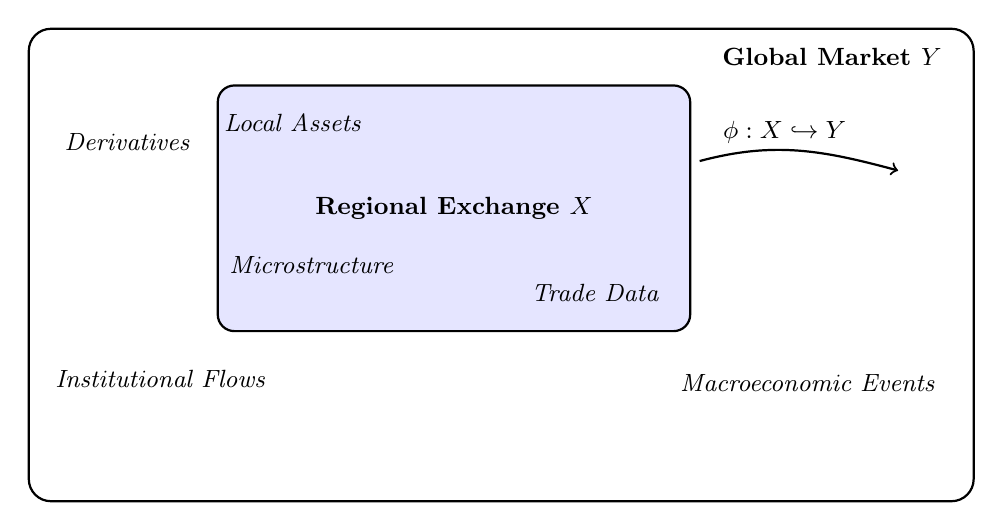
\begin{tikzpicture}[scale=1.2, every node/.style={font=\small}]
    % Global market Y
    \draw[thick, rounded corners=8pt] (0,0) rectangle (10,5);
    \node at (8.5,4.7) {\textbf{Global Market \(\boldsymbol{Y}\)}};

    % Enlarged Regional exchange X
    \draw[thick, fill=blue!10, rounded corners=6pt] (2,1.8) rectangle (7,4.4);
    \node at (4.5,3.1) {\textbf{Regional Exchange \(\boldsymbol{X}\)}};

    % Assets in X
    \node at (2.8,4.0) {\textit{Local Assets}};
    \node at (3.0,2.5) {\textit{Microstructure}};
    \node at (6.0,2.2) {\textit{Trade Data}};

    % Assets outside X (in Y)
    \node at (1.4,1.3) {\textit{Institutional Flows}};
    \node at (1.05,3.8) {\textit{Derivatives}};
    \node at (8.25,1.25) {\textit{Macroeconomic Events}};

    % Arrow to show embedding
    \draw[->, thick] (7.1,3.6) to[out=15,in=165] (9.2,3.5);
    \node at (8,3.9) {\(\phi: X \hookrightarrow Y\)};

\end{tikzpicture}
\caption{The regional exchange \( X \) is embedded within the global market \( Y \), preserving structure and measure through an inclusion map.}
\end{figure}



Crucially, when incorporating the regional data into the global market model, you don’t want to distort anything. A \$10 million trade on the local exchange should still count as a \$10 million trade in the global context. The events are not transformed or rescaled; they are simply recognized as part of a larger universe. This process is what an \textbf{inclusion map} formalizes: it preserves the structure and significance (i.e., the measure) of local information while embedding it into a wider context.

\begin{figure}[H]
\centering
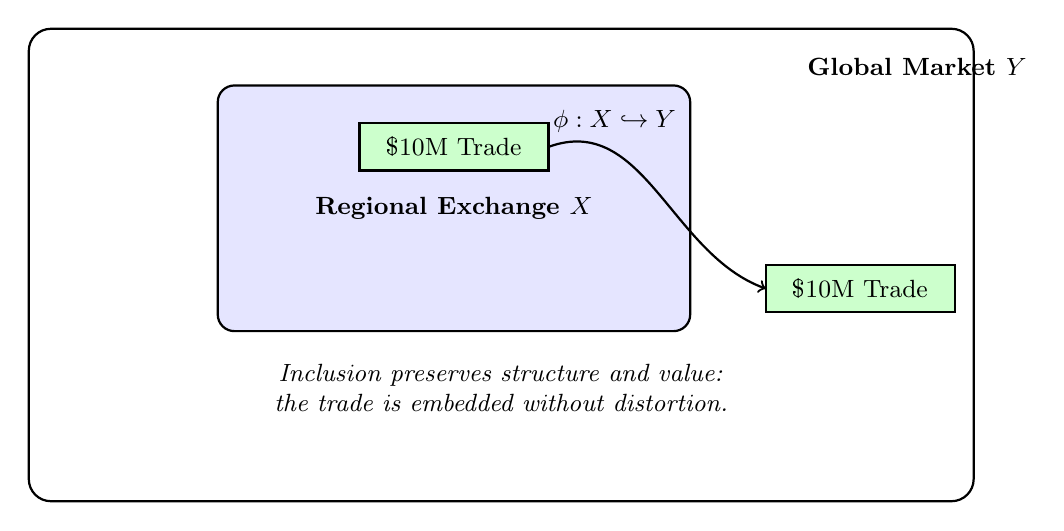
\begin{tikzpicture}[scale=1.2, every node/.style={font=\small}]

    % Global Market Y
    \draw[thick, rounded corners=8pt] (0,0) rectangle (10,5);
    \node at (9.4,4.6) {\textbf{Global Market \(\boldsymbol{Y}\)}};

    % Regional Exchange X (larger inner rectangle)
    \draw[thick, fill=blue!10, rounded corners=6pt] (2,1.8) rectangle (7,4.4);
    \node at (4.5,3.1) {\textbf{Regional Exchange \(\boldsymbol{X}\)}};

    % Example Trade inside X
    \draw[fill=green!20, thick] (3.5,3.5) rectangle (5.5,4.0);
    \node at (4.5,3.75) {\$10M Trade};

    % Trade copy inside Y (mirrored)
    \draw[fill=green!20, thick] (7.8,2.0) rectangle (9.8,2.5);
    \node at (8.8,2.25) {\$10M Trade};

    % Arrow representing inclusion
    \draw[->, thick] (5.5,3.75) to[out=20,in=160] (7.8,2.25);
    \node[above] at (6.2,3.8) {\(\phi: X \hookrightarrow Y\)};

    % Annotation
    \node[align=center] at (5,1.2) {
        \textit{Inclusion preserves structure and value:} \\
        \textit{the trade is embedded without distortion.}
    };

\end{tikzpicture}
\caption{An inclusion map embeds local data into a global system without distortion: a \$10 million trade in the regional market remains a \$10 million trade in the global model.}
\end{figure}


\vspace{1em}
Formally, given two measure spaces \( (X, \mathcal{F}_X, \mu_X) \) and \( (Y, \mathcal{F}_Y, \mu_Y) \), an \textbf{inclusion map} is defined as:

\[
\phi: X \hookrightarrow Y, \quad \phi(x) = x, \quad \forall x \in X.
\]

This simply means that each element of \( X \) is mapped to itself in \( Y \), preserving identity. The key property is that the measure of any subset \( A \subset X \) remains unchanged:

\[
\mu_X(A) = \mu_Y(\phi(A)).
\]


\begin{figure}[H]
\centering
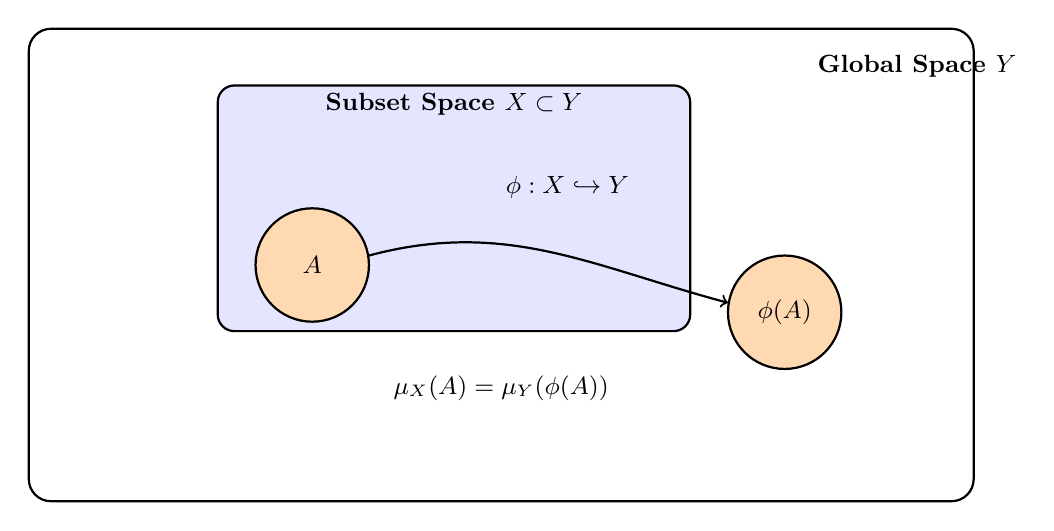
\begin{tikzpicture}[scale=1.2, every node/.style={font=\small}]

    % Global Market Y
    \draw[thick, rounded corners=8pt] (0,0) rectangle (10,5);
    \node at (9.4,4.6) {\textbf{Global Space \( Y \)}};

    % Regional Exchange X
    \draw[thick, fill=blue!10, rounded corners=6pt] (2,1.8) rectangle (7,4.4);
    \node at (4.5,4.2) {\textbf{Subset Space \( X \subset Y \)}};

    % Subset A inside X
    \draw[fill=orange!30, thick] (3,2.5) circle (0.6);
    \node at (3,2.5) {\( A \)};

    % Corresponding subset φ(A) in Y
    \draw[fill=orange!30, thick] (8,2.0) circle (0.6);
    \node at (8,2.0) {\( \phi(A) \)};

    % Arrow showing inclusion map
    \draw[->, thick] (3.6,2.6) to[out=15,in=165] (7.4,2.1);
    \node[above] at (5.7,3.1) {\(\phi: X \hookrightarrow Y\)};

    % Measure equivalence annotation
    \node at (5,1.2) {\(\mu_X(A) = \mu_Y(\phi(A))\)};

\end{tikzpicture}
\caption{An inclusion map preserves both identity and measure: a subset \( A \subset X \) retains its importance when mapped into the larger space \( Y \).}
\end{figure}

In other words, the importance (or probability, or volume) assigned to events in the smaller space \( X \) remains intact when viewed from the larger space \( Y \). For financial modeling, this allows us to combine local and global perspectives without distorting the quantitative meaning of the data.

\vspace{1em}
\noindent
To bridge the abstract concept of inclusion maps with a concrete setting, we model both the regional exchange \( X \) and the global market \( Y \) as partially ordered sets. Events in \( X \) — such as trades or price updates — are elements of a poset reflecting their causal relationships. When these events are embedded into \( Y \), they preserve their structure, but \( Y \) may contain additional events and interactions not visible within the scope of \( X \).

This Hasse diagram shows how a subset of global market events (in blue) corresponds to the local system \( X \), while additional global events (in green) reflect broader market dynamics. The inclusion map \( \phi: X \hookrightarrow Y \) embeds each event \( x_i \in X \) into its global counterpart \( y_i = \phi(x_i) \in Y \), maintaining causal structure without distorting the relationships or values.

\begin{figure}[H]
\centering
\begin{tikzpicture}[
    xevent/.style={circle, draw=black, fill=blue!10, thick, minimum size=1.2cm},
    yevent/.style={circle, draw=black, fill=green!10, thick, minimum size=1.2cm},
    arrow/.style={-Stealth, thick},
    dashedarrow/.style={->, thick, dashed, gray},
    node distance=1.5cm and 2cm,
    every node/.style={font=\small}
]

% Events in X (subset)
\node[xevent] (x1) at (0,0) {\( x_1 \)};
\node[xevent, above left=of x1] (x2) {\( x_2 \)};
\node[xevent, above=of x2] (x4) {\( x_4 \)};

% Arrows in X
\draw[arrow] (x1) -- (x2);
\draw[arrow] (x2) -- (x4);

% Events in Y (superset)
\node[yevent, right=5cm of x1] (y1) {\( y_1 \)};
\node[yevent, above left=of y1] (y2) {\( y_2 \)};
\node[yevent, above=of y2] (y4) {\( y_4 \)};
\node[yevent, above right=of y1, xshift=0.4cm] (y3) {\( y_3 \)};
\node[yevent, above=of y3] (y5) {\( y_5 \)};

% Arrows in Y
\draw[arrow] (y1) -- (y2);
\draw[arrow] (y2) -- (y4);
\draw[arrow] (y1) -- (y3);
\draw[arrow] (y3) -- (y5);

% Inclusion map arrows
\draw[dashedarrow] (x1) -- (y1);
\draw[dashedarrow] (x2) -- (y2);
\draw[dashedarrow] (x4) -- (y4);

% Labels
\node at (-1.5,3.5) {\textbf{Regional Exchange \( X \)}};
\node at (6.5,4.5) {\textbf{Global Market \( Y \)}};
\node at (0.7,2.5) {\( \phi: X \hookrightarrow Y \)};

\end{tikzpicture}
\caption{A subset of causally ordered events in the regional exchange \( X \) is embedded into the global market \( Y \) via the inclusion map \( \phi \). Events \( y_3 \) and \( y_5 \) are present in \( Y \) but not in \( X \), showing that \( X \subset Y \) captures only part of the full system.}
\end{figure}

\vspace{1em}
\noindent
So the next time someone insists their regional trading model "totally captures the global dynamics," you can smile, point to your inclusion map, and gently remind them: “Yes, your trades exist — but only as a proper subset.” Because in finance, as in mathematics, knowing where you fit in the larger $\sigma$-algebra is half the battle.



\begin{figure}[H]
\centering
\begin{tikzpicture}[every node/.style={font=\footnotesize}]

% Panel 1 — Analyst 1 confused
\comicpanel{0}{4}
  {Analyst 1}
  {Analyst 2}
  {So if we move a \$10M trade from the regional market to the global model... do we rescale it? Reclassify it? Normalize it?}
  {(0,-0.6)}

% Panel 2 — Analyst 2 clarifies
\comicpanel{6.5}{4}
  {Analyst 1}
  {Analyst 2}
  {Nope. It's still a \$10M trade. We’re not doing financial alchemy here.}
  {(0,-0.5)}

% Panel 3 — Analyst 1 leans in
\comicpanel{0}{0}
  {Analyst 1}
  {Analyst 2}
  {But surely the macro context gives it more... global aura? Maybe a currency glow effect?}
  {(0,0.6)}

% Panel 4 — Analyst 2 delivers punchline
\comicpanel{6.5}{0}
  {Analyst 1}
  {Analyst 2}
  {It’s an inclusion map. Not a magical realism filter.}
  {(0,0.6)}

\end{tikzpicture}
\caption{Inclusion maps: preserving meaning without market mysticism.}
\end{figure}







\subsection{Application to High-Frequency Trading}

\vspace{0.5em}
\noindent
Building on the idea of inclusion maps from the previous section, let’s zoom in on a high-frequency trading scenario. Imagine you’re watching a trading algorithm that repeatedly places rapid-fire trades. Each time it does, you observe a corresponding movement in the market price. It’s tempting to conclude that the trades are causing the price change — this would suggest a direct inclusion: the set of trades is embedded within the set of price changes.

But then you look closer. It turns out both the algorithm and the price movement tend to react to something else entirely ; like the release of government unemployment data or a sudden institutional sell-off. In this case, the trades and price movements are not causally linked to each other but are both effects of a third, hidden cause. If you mistakenly assume a direct inclusion, your model will identify spurious causality and could lead to catastrophic mispricing under stress.

This is where inclusion maps become more than just abstract math: they provide a framework to rigorously distinguish between real causation and mere coincidence in complex systems like financial markets.

\vspace{1em}
We model the entire market as a \textbf{measurable space} \( (\Omega, \mathcal{F}, \mu) \), where:

\begin{itemize}
    \item \( \Omega \) is the universe of all possible micro-events in the market — including trades, price updates, order book shifts, and macroeconomic announcements.
    
    \item \( \mathcal{F} \subset 2^\Omega \) is the \textbf{sigma-algebra} of measurable events: it contains all the collections of market events that are observable and well-defined in terms of market structure (e.g., "all trades within a 10ms window after a news release").
    
    \item \( \mu: \mathcal{F} \rightarrow [0, \infty] \) is a \textbf{measure} that assigns weight to each measurable set — such as trade volume, probability of occurrence, or economic significance. This allows us to compare and reason about the importance or likelihood of different events within the market.

    \item \( S \subset \Omega \) is the set of trades executed by a specific machine or algorithm.

    \item \( T \subset \Omega \) is the set of observed price changes across the market.

    \item \( C \subset \Omega \) is the \textbf{true causal set} — macroeconomic events such as central bank announcements, liquidity shocks, or institutional actions that influence both \( S \) and \( T \).
\end{itemize}

\begin{figure}[H]
\centering
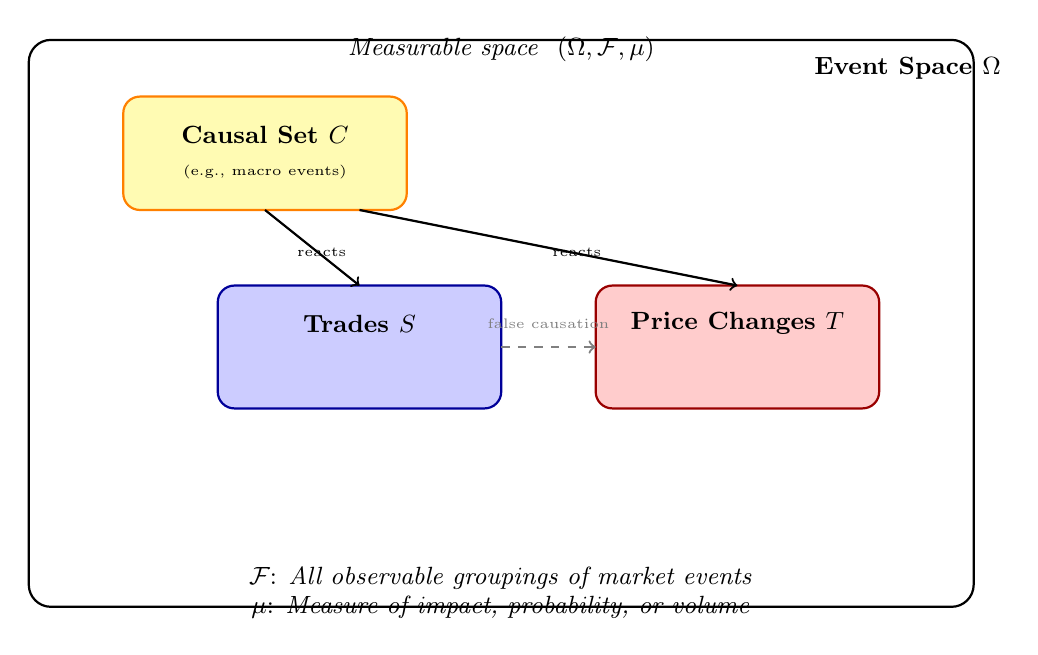
\begin{tikzpicture}[scale=1.2, every node/.style={font=\small}]

    % Universal measurable space Omega
    \draw[thick, rounded corners=8pt] (0,0) rectangle (10,6);
    \node at (9.3,5.7) {\textbf{Event Space \(\Omega\)}};
    \node at (5,5.9) {\textit{Measurable space } \(\boldsymbol{(\Omega, \mathcal{F}, \mu)}\)};
    
    % Label sigma-algebra
    \node at (5,0.3) {\(\mathcal{F}\): \textit{All observable groupings of market events}};
    
    % Label measure
    \node at (5,0.0) {\(\mu\): \textit{Measure of impact, probability, or volume}};

    % Subset C — True causal set
    \draw[fill=yellow!30, draw=orange, thick, rounded corners=6pt] (1,4.2) rectangle (4,5.4);
    \node at (2.5,5.0) {\textbf{Causal Set \(C\)}};
    \node at (2.5,4.6) {\tiny (e.g., macro events)};

    % Subset S — Trades
    \draw[fill=blue!20, draw=blue!60!black, thick, rounded corners=6pt] (2,2.1) rectangle (5,3.4);
    \node at (3.5,3.0) {\textbf{Trades \(S\)}};

    % Subset T — Price Changes
    \draw[fill=red!20, draw=red!60!black, thick, rounded corners=6pt] (6,2.1) rectangle (9,3.4);
    \node at (7.5,3.0) {\textbf{Price Changes \(T\)}};

    % Arrows from C to S and T
    \draw[->, thick] (2.5,4.2) -- (3.5,3.4);
    \draw[->, thick] (3.5,4.2) -- (7.5,3.4);
    \node at (3.1,3.75) {\tiny reacts};
    \node at (5.8,3.75) {\tiny reacts};

    % Dashed arrow for false assumption
    \draw[->, thick, dashed, gray] (5,2.75) -- (6,2.75);
    \node[gray] at (5.5,3.0) {\tiny false causation};

\end{tikzpicture}
\caption{The market is modeled as a measurable space \( (\Omega, \mathcal{F}, \mu) \), where trades \( S \) and price changes \( T \) are observable events. Both may appear related, but are often reactions to a deeper causal set \( C \).}
\end{figure}


If trades genuinely cause price changes, we expect an inclusion map of the form:

\[
\phi: S \hookrightarrow T.
\]

\begin{figure}[H]
\centering
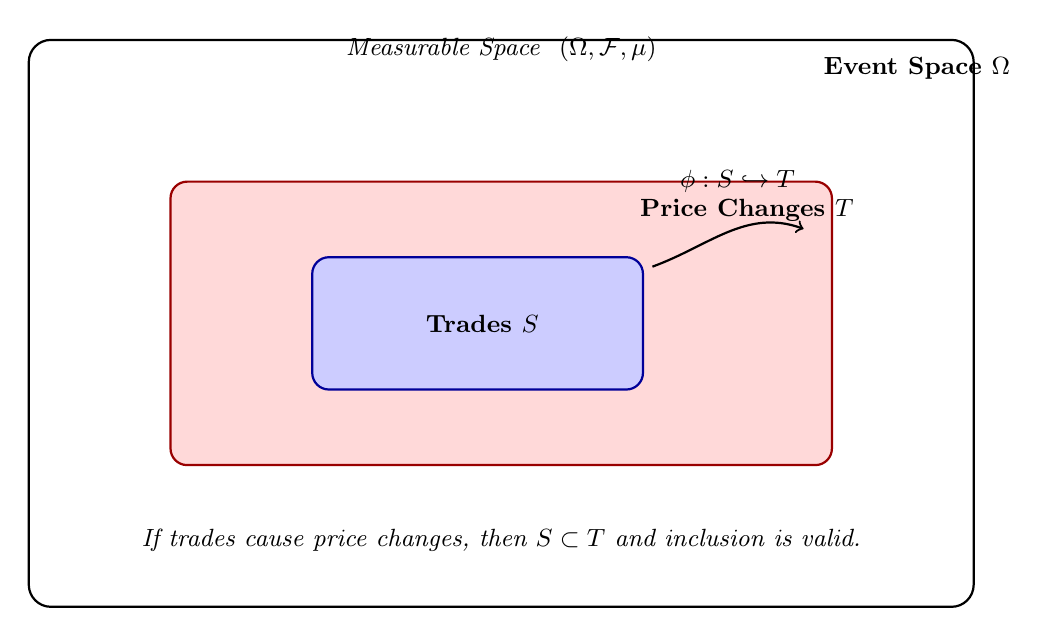
\begin{tikzpicture}[scale=1.2, every node/.style={font=\small}]

    % Universal space Omega
    \draw[thick, rounded corners=8pt] (0,0) rectangle (10,6);
    \node at (9.4,5.7) {\textbf{Event Space \(\Omega\)}};
    \node at (5,5.9) {\textit{Measurable Space } \((\Omega, \mathcal{F}, \mu)\)};

    % Subset T (Price Changes)
    \draw[fill=red!15, draw=red!60!black, thick, rounded corners=6pt] (1.5,1.5) rectangle (8.5,4.5);
    \node at (7.6,4.2) {\textbf{Price Changes \(T\)}};

    % Subset S inside T (Trades)
    \draw[fill=blue!20, draw=blue!60!black, thick, rounded corners=6pt] (3,2.3) rectangle (6.5,3.7);
    \node at (4.8,3.0) {\textbf{Trades \(S\)}};

    % Arrow annotation showing inclusion map
    \draw[->, thick] (6.6,3.6) to[out=20,in=160] (8.2,4.0);
    \node at (7.5,4.5) {\(\phi: S \hookrightarrow T\)};

    % Annotation
    \node at (5,0.7) {\textit{If trades cause price changes, then \( S \subset T \) and inclusion is valid.}};

\end{tikzpicture}
\caption{When trades \( S \) genuinely cause price changes \( T \), both are subsets of the market event space \( \Omega \), and the inclusion map \( \phi: S \hookrightarrow T \) correctly captures the causal structure.}
\end{figure}


This means the measure on trade activity naturally embeds within the measure on price movement. However, if both \( S \) and \( T \) are merely responding to \( C \), then the more accurate inclusion is:

\[
\phi: S \hookrightarrow \Omega \setminus C.
\]


\begin{figure}[H]
\centering
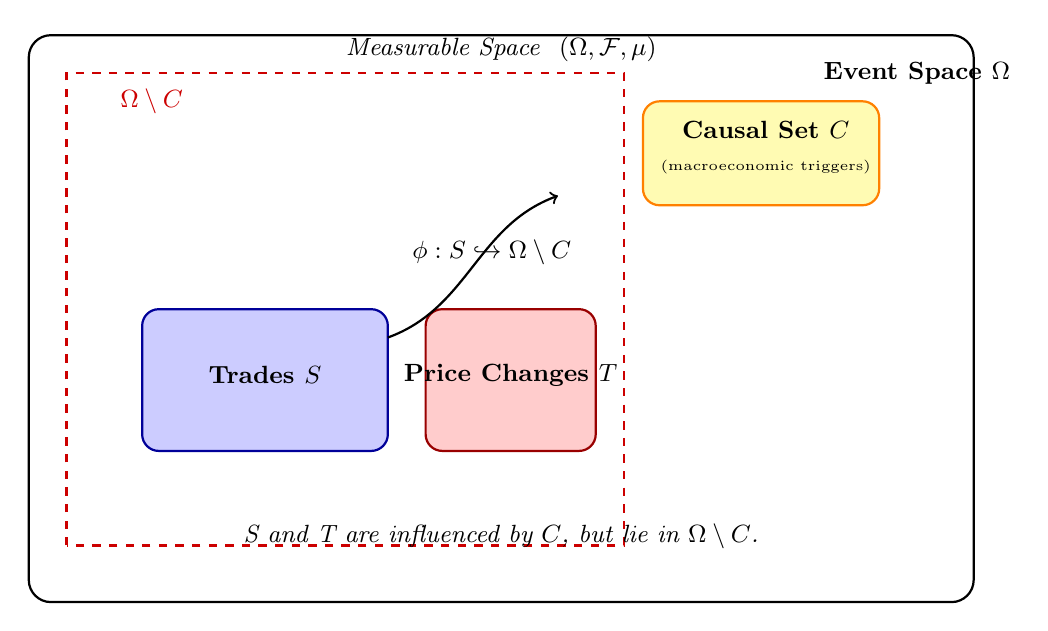
\begin{tikzpicture}[scale=1.2, every node/.style={font=\small}]

    % Full Event Space Omega
    \draw[thick, rounded corners=8pt] (0,0) rectangle (10,6);
    \node at (9.4,5.6) {\textbf{Event Space \(\Omega\)}};
    \node at (5,5.85) {\textit{Measurable Space } \((\Omega, \mathcal{F}, \mu)\)};

    % Subset C — True Causal Set (Should NOT be inside Omega \ C)
    \draw[fill=yellow!30, draw=orange, thick, rounded corners=6pt] (6.5,4.2) rectangle (9,5.3);
    \node at (7.8,5.0) {\textbf{Causal Set \(C\)}};
    \node at (7.8,4.6) {\tiny (macroeconomic triggers)};

    % Highlighted dashed box for Omega \ C (excludes C visually)
    \draw[dashed, thick, red!80!black] (0.4,0.6) rectangle (6.3,5.6);
    \node[red!80!black] at (1.3,5.3) {\(\Omega \setminus C\)};

    % Subset S — Trades (inside Omega \ C)
    \draw[fill=blue!20, draw=blue!60!black, thick, rounded corners=6pt] (1.2,1.6) rectangle (3.8,3.1);
    \node at (2.5,2.4) {\textbf{Trades \(S\)}};

    % Subset T — Price Changes (also inside Omega \ C)
    \draw[fill=red!20, draw=red!60!black, thick, rounded corners=6pt] (4.2,1.6) rectangle (6.0,3.1);
    \node at (5.1,2.4) {\textbf{Price Changes \(T\)}};

    % Inclusion arrow from S to Omega \ C (not pointing into C)
    \draw[->, thick] (3.8,2.8) to[out=20,in=200] (5.6,4.3);
    \node at (4.9,3.7) {\(\phi: S \hookrightarrow \Omega \setminus C\)};

    % Annotation
    \node at (5,0.7) {\textit{S and T are influenced by \(C\), but lie in \(\Omega \setminus C\).}};

\end{tikzpicture}
\caption{When both trades \( S \) and price changes \( T \) are effects of a hidden cause \( C \), the correct inclusion is \( \phi: S \hookrightarrow \Omega \setminus C \), which avoids misinterpreting correlation as causation.}
\end{figure}

\vspace{1em}
\noindent
\textbf{Why is \( T \) inside \( \Omega \setminus C \)?}

\vspace{0.5em}
When we write \( \phi: S \hookrightarrow \Omega \setminus C \), we are stating that the set of trades \( S \) belongs to the portion of the event space that excludes the causal set \( C \). If we believe that price changes \( T \) are also \emph{effects} of the true cause \( C \) — not directly caused by \( S \) — then \( T \) too should be located in \( \Omega \setminus C \). 

This means both \( S \) and \( T \) are valid elements of the same subset space, avoiding the erroneous assumption that one causes the other. However, they are still part of the full market space \( \Omega \). The diagram reflects this correctly.

\vspace{1em}
\begin{center}
\renewcommand{\arraystretch}{1.3}
\begin{tabular}{|c|p{8cm}|}
\hline
\textbf{Set} & \textbf{Meaning and Placement} \\
\hline
\( \Omega \) & The complete market event space; contains everything. Represented by the large outer rectangle. \\
\hline
\( C \subset \Omega \) & The true causal set (e.g., macroeconomic events). Placed inside \( \Omega \), but outside of \( \Omega \setminus C \). \\
\hline
\( \Omega \setminus C \) & The complement of the causal set within \( \Omega \); contains events not caused by \( C \). Represented by the dashed bounding box. \\
\hline
\( S, T \subset \Omega \setminus C \) & The sets of trades and price changes, both outside of \( C \) but still within \( \Omega \). Placed inside the dashed box and outside \( C \). \\
\hline
\end{tabular}
\end{center}

\vspace{1em}
\noindent
\textit{Conclusion:} To claim \( \phi: S \hookrightarrow \Omega \setminus C \), both \( S \) and \( T \) must be subsets of \( \Omega \setminus C \), not of \( C \). The diagram reflects this structure correctly.





This measure-theoretic perspective helps separate signal from noise — and more importantly, causation from correlation — in the rapid-fire, feedback-heavy world of algorithmic trading.


\subsubsection*{Concrete Example: Misinterpreting Causality in Event Ordering}

To make this abstract framework more tangible, consider a simple sequence of events in a high-frequency trading system. A machine places a trade. Shortly after, the price moves. At first glance, this seems like causation: the trade appears to drive the price.

However, suppose that just before both of these events, a macroeconomic indicator was released — triggering both the trade and the price movement. If we model this situation using event orderings, we see that the trade and price change are not causally linked to each other, but both follow from a third event.

The Hasse diagram below shows this structure clearly: the macroeconomic trigger \( c \) precedes both the trade \( s \) and the price update \( t \), but there's no direct causal path from \( s \) to \( t \). Mistaking this configuration as \( s \rightarrow t \) would be a case of false causation.


\begin{figure}[H]
\centering
\begin{tikzpicture}[
    node distance=1.5cm and 2.2cm,
    event/.style={circle, draw=black, fill=blue!10, thick, minimum size=1.2cm},
    arrow/.style={-Stealth, thick},
    every node/.style={font=\small}
]

% Nodes
\node[event] (c) at (0,2.5) {\( c \)};
\node[event, below left=of c] (s) {\( s \)};
\node[event, below right=of c] (t) {\( t \)};

% Arrows from cause to both
\draw[arrow] (c) -- (s);
\draw[arrow] (c) -- (t);

% Label
\node at (0,3.5) {\textbf{Causal Hasse Diagram}};

\end{tikzpicture}
\caption{Macroeconomic event \( c \) causes both the trade \( s \) and price change \( t \), but \( s \) and \( t \) are not causally linked. Misinterpreting this structure leads to false attribution of causality.}
\end{figure}


\vspace{1em}
\noindent
Models that ignore hidden causes often return elegant, confident conclusions — right up until the market reminds us that elegance without causality is just curve-fitting in a tuxedo. In high-frequency trading, where every microsecond invites misinterpretation, inclusion maps and measure-theoretic reasoning don’t just clarify structure — they keep us from hallucinating ghosts in the data.



\begin{figure}[H]
\centering
\begin{tikzpicture}[every node/.style={font=\footnotesize}]

% Panel 1 — Algo trader excited
\comicpanel{0}{4}
  {Algo A}
  {Algo B}
  {Did you see that? I placed a trade and boom — price moved. Clearly I caused it.}
  {(-0.3,-0.6)}

% Panel 2 — Algo B skeptical
\comicpanel{6.5}{4}
  {Algo A}
  {Algo B}
  {Or maybe we both reacted to that unemployment report. Ever think of that?}
  {(-0.2,-0.6)}

% Panel 3 — Algo A tries to justify
\comicpanel{0}{0}
  {Algo A}
  {Algo C}
  {I mean, sure... but the inclusion felt real. It was a very includable moment.}
  {(0,0.5)}

% Panel 4 — Algo C brings the math
\comicpanel{6.5}{0}
  {Algo A}
  {Algo C}
  {Check your inclusion map. You're inside \(\Omega \setminus C\), not inside price movement.}
  {(0,0.6)}

\end{tikzpicture}
\caption{Spurious causality: when your trades look important, but are just echoes of macro events.}
\end{figure}


\subsection{Mutual Information and Inclusion Maps}

\subsubsection{From Correlation to Causation: A Role for Mutual Information}

\vspace{0.5em}
\noindent
Continuing from the previous section, let’s say you've built an inclusion map that seems to link a trading algorithm’s actions to market price movements. You notice a pattern: whenever the algorithm places a flurry of trades, the price moves shortly afterward. At first glance, this looks like a strong signal that the trades might be driving the market.

But you're not convinced. You wonder: is this real causation, or are both just reacting to something else? Maybe a government report just dropped, or maybe a large institutional trader moved the market before your algorithm even fired. You want a tool that quantifies how strong the relationship is, and how much of it disappears once you account for external influences.

That tool is mutual information. It tells you how much knowing one variable (like trade activity) reduces uncertainty about another (like price changes). Even better, by conditioning on a potential confounder — say, macroeconomic news — you can test whether the relationship still holds or falls apart.

\subsubsection{Mutual Information as a Correction to Maximum Entropy}

\vspace{0.5em}
\noindent
We start with \textbf{maximum entropy}: a position of total uncertainty, assuming that trades, prices, and external events are all independent. Mutual information acts as a correction to this ignorance. If observing trades significantly reduces your uncertainty about price movements, you gain mutual information — a signal that a dependency exists. But if conditioning on a shared external cause eliminates that dependency, it reveals the relationship as spurious.

\begin{figure}[H]
\centering
\begin{tikzpicture}[
    node distance=2.2cm and 2.8cm,
    var/.style={circle, draw, thick, minimum size=1.3cm, align=center},
    info/.style={rectangle, draw, thick, rounded corners, fill=gray!10, inner sep=8pt, text width=6cm},
    arrow/.style={->, thick, >=Stealth}
]

% Nodes
\node[var] (trades) {Trades};
\node[var, right=of trades] (price) {Price};
\node[var, above=of $(trades)!0.5!(price)$] (external) {External\\Events};

% Arrows
\draw[arrow] (trades) -- (price);
\draw[arrow, dashed] (external) -- (trades);
\draw[arrow, dashed] (external) -- (price);

% Annotation box
\node[info, below=1.5cm of $(trades)!0.5!(price)$] (annotation) {
  \textbf{Mutual Information:}\\
  How much does knowing Trades reduce uncertainty about Price?\\
  \vspace{0.4em}
  \textbf{Conditioning:}\\
  If External Events explain both, the dependency might vanish.
};

\end{tikzpicture}
\caption{Illustration of mutual information between Trades and Price, with potential confounding from External Events.}
\end{figure}

\noindent
This diagram begins from a state of maximum entropy — a world where trades, prices, and external events are assumed independent. Mutual information measures how far reality deviates from that assumption. If observing trades helps predict price changes, mutual information reveals a dependency. But the presence of a shared external influence can create the illusion of causality. By conditioning on this influence, we can test whether the dependency is real or spurious.

\begin{center}
\renewcommand{\arraystretch}{1.4}
\begin{tabular}{|p{5.2cm}|p{7.4cm}|}
\hline
\textbf{Concept} & \textbf{Visual Representation} \\
\hline
Trades and Prices are linked & Solid arrow from Trades to Price \\
\hline
External Events influence both & Dashed arrows from External Events to both Trades and Price \\
\hline
Mutual Information detects a dependency & Shown as the implied flow from Trades to Price via information reduction \\
\hline
Conditioning reveals deeper structure & If the dashed arrows explain away the solid one, the dependency may be spurious \\
\hline
\end{tabular}
\end{center}

\vspace{1em}
\noindent
This sets the stage for using mutual information not only to detect potential links, but to interrogate them — separating causation from correlation in reactive environments like markets.


\subsubsection{Quantifying Dependence via Entropy}



\vspace{1em}
\noindent
Formally, mutual information between trades \( S \) and price changes \( T \) is defined as:

\[
I(S; T) = H(S) + H(T) - H(S, T),
\]

where \( H(S) \) and \( H(T) \) are the entropies of the two variables, and \( H(S, T) \) is their joint entropy. This measures how much uncertainty is reduced by observing both together, compared to treating them separately.

\begin{figure}[H]
\centering
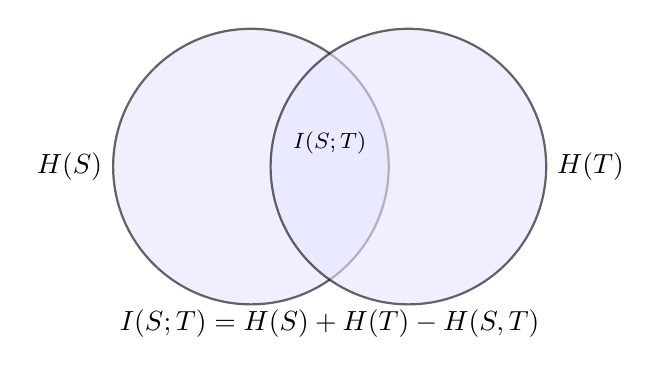
\begin{tikzpicture}[
    entropy/.style={circle, minimum width=3.5cm, draw=black, thick, fill=blue!10, opacity=0.6},
    entropylabel/.style={font=\footnotesize\bfseries},
]

% Entropy circles with more overlap
\node[entropy, label=left:\( H(S) \)] (HS) at (0,0) {};
\node[entropy, label=right:\( H(T) \)] (HT) at (2,0) {};

% Mutual information label centered in overlap
\node[entropylabel] at (1, 0.3) {\( I(S; T) \)};

% Equation below
\node at (1, -2) {\( I(S; T) = H(S) + H(T) - H(S, T) \)};

\end{tikzpicture}
\caption{Visualizing mutual information as the overlap between the entropies of Trades \( S \) and Prices \( T \).}
\end{figure}

\noindent
This diagram shows how mutual information quantifies the reduction in uncertainty when observing two variables together. Here, trades \( S \) and price changes \( T \) are represented as overlapping uncertainty sets. Their mutual information is the part that is shared — the reduction in unpredictability one provides about the other.

\begin{center}
\renewcommand{\arraystretch}{1.4}
\begin{tabular}{|p{5.2cm}|p{7.4cm}|}
\hline
\textbf{Concept} & \textbf{Visual Representation} \\
\hline
Uncertainty in trades \( S \) & Entire area of circle labeled \( H(S) \) \\
\hline
Uncertainty in price changes \( T \) & Entire area of circle labeled \( H(T) \) \\
\hline
Joint uncertainty in observing both together & Union of both circles, corresponding to \( H(S, T) \) \\
\hline
Mutual information \( I(S; T) \) & Overlapping region — the shared information between \( S \) and \( T \) \\
\hline
\end{tabular}
\end{center}

\vspace{1em}
\noindent
This formalizes the intuition that mutual information tells us how much knowing one variable informs us about the other — and how far the world is from total independence.


\subsubsection{Testing for Causality with Conditional Mutual Information}


To test for causality, we condition on the hidden causal set \( C \). If the dependency between \( S \) and \( T \) is real, mutual information should remain intact:

\[
I(S; T \mid C) \approx I(S; T).
\]

\begin{figure}[H]
\centering
\begin{tikzpicture}[
    entropy/.style={circle, minimum width=3.5cm, draw=black, thick, fill=blue!10, opacity=0.6},
    condition/.style={ellipse, minimum width=6.2cm, minimum height=4cm, draw=red!70!black, thick, dashed, fill=red!10, opacity=0.3},
    labelstyle/.style={font=\footnotesize\bfseries}
]

% Entropy circles
\node[entropy, label=left:\( H(S) \)] (HS) at (0,0) {};
\node[entropy, label=right:\( H(T) \)] (HT) at (2,0) {};

% Conditioning set as a dashed ellipse around both
\node[condition, label={[labelstyle]above:\( C \)}] (C) at (1,0) {};

% Mutual information label in overlap
\node[labelstyle] at (1, 0.3) {\( I(S; T \mid C) \)};

% Equation below
\node at (1, -2.2) {\( I(S; T \mid C) \approx I(S; T) \Rightarrow \) likely causality};

\end{tikzpicture}
\caption{Conditional mutual information: If the dependency between \( S \) (Trades) and \( T \) (Price) persists when conditioned on \( C \) (Hidden Causes), it's likely causal.}
\end{figure}

\noindent
This diagram illustrates the scenario where the relationship between trades \( S \) and price movements \( T \) likely reflects a real causal influence. The visual elements and their meanings are summarized below:

\begin{center}
\renewcommand{\arraystretch}{1.4}
\begin{tabular}{|p{5.2cm}|p{7.4cm}|}
\hline
\textbf{Concept} & \textbf{Visual Representation} \\
\hline
\( S \) and \( T \) are both influenced by \( C \), but retain a direct link & The conditioning set \( C \) overlaps with both entropy sets \( H(S) \) and \( H(T) \), but does not eliminate their overlap \\
\hline
A persistent dependency remains between \( S \) and \( T \) after conditioning & The entropy circles \( H(S) \) and \( H(T) \) still overlap inside \( C \) \\
\hline
\( I(S; T \mid C) \approx I(S; T) \) & Conditioning on \( C \) does not reduce the mutual information — suggesting a likely causal connection \\
\hline
\end{tabular}
\end{center}

\vspace{1em}
\noindent
Mutual information, when preserved after conditioning on a shared cause, becomes strong evidence for a genuine interaction — a possible causal influence rather than a coincidental correlation.

\subsubsection{When Conditional Mutual Information Vanishes}



But if \( S \) and \( T \) are both simply reacting to \( C \), then conditioning removes the apparent dependency:

\[
I(S; T \mid C) \approx 0.
\]

This tells us that the correlation between trades and price movement was an illusion since both were echoes of something deeper. Mutual information, then, becomes a tool not just for detection, but for validation of causality in noisy, reactive systems like financial markets.

\begin{figure}[H]
\centering
\begin{tikzpicture}[
    entropy/.style={circle, minimum width=3.5cm, draw=black, thick, fill=blue!10, opacity=0.6},
    condition/.style={ellipse, minimum width=7cm, minimum height=4cm, draw=red!70!black, thick, dashed, fill=red!10, opacity=0.3},
    labelstyle/.style={font=\footnotesize\bfseries}
]

% Properly disjoint entropy circles
\node[entropy, label=left:\( H(S) \)] (HS) at (0,0) {};
\node[entropy, label=right:\( H(T) \)] (HT) at (4,0) {};

% Conditioning set
\node[condition, label={[labelstyle]above:\( C \)}] (C) at (2,0) {};

% Label indicating no mutual information
\node[labelstyle] at (2, 0.3) {\( I(S; T \mid C) \approx 0 \)};

% Explanation below
\node at (2, -2.2) {\parbox{8cm}{\centering Conditioning on \( C \) removes the apparent dependency.\\ No true causality — just a shared response to a hidden driver.}};

\end{tikzpicture}
\caption{When mutual information disappears after conditioning, the apparent link between Trades \( S \) and Price \( T \) was spurious.}
\end{figure}

\noindent
The illustration shows how conditioning on a hidden cause \( C \) affects the apparent relationship between trades \( S \) and price movements \( T \). The key visual elements and their meanings are summarized below:

\begin{center}
\renewcommand{\arraystretch}{1.4}
\begin{tabular}{|p{5.2cm}|p{7.4cm}|}
\hline
\textbf{Concept} & \textbf{Visual Representation} \\
\hline
\( S \) and \( T \) are influenced by \( C \) & The conditioning set \( C \) overlaps with both entropy sets \( H(S) \) and \( H(T) \) \\
\hline
No direct dependency between \( S \) and \( T \) after conditioning & \( H(S) \) and \( H(T) \) are disjoint (no overlap between circles) \\
\hline
\( I(S; T \mid C) \approx 0 \) & The mutual information region disappears; conditioning on \( C \) explains away the correlation \\
\hline
\end{tabular}
\end{center}

\vspace{1em}
\noindent
This illustrates how mutual information helps distinguish between causal influence and mere co-responsiveness to an external factor in reactive systems like financial markets.




\subsubsection{A Concrete Example: An Algorithm, a Price Spike, and a False Alarm}

\vspace{0.5em}
\noindent
Let’s say you're monitoring a high-frequency trading algorithm — call it \texttt{AlphaFlash}. It's designed to detect short-term inefficiencies in the spread between two correlated assets. On several occasions, you notice the following pattern:

\begin{itemize}
    \item \texttt{AlphaFlash} fires a rapid burst of trades around time \( t_0 \).
    \item Within milliseconds, the market price ticks upward.
\end{itemize}

It looks like textbook causality: a trade causes a price impact. Mutual information between the trade signals \( S \) and the price updates \( T \) is significantly positive:

\[
I(S; T) > 0.
\]

But then you add a new data stream into your analysis: a real-time economic feed. On closer inspection, you find that every instance of this pattern was preceded by the publication of a central bank policy announcement — a hidden variable \( C \) that affects both trade behavior and market prices.

After conditioning on \( C \), the mutual information nearly vanishes:

\[
I(S; T \mid C) \approx 0.
\]

This reveals a spurious correlation. The algorithm and the market weren’t responding to each other; they were both responding to \( C \).

\begin{figure}[H]
\centering
\begin{tikzpicture}[
    event/.style={circle, draw=black, thick, minimum size=1.2cm, align=center},
    arrow/.style={->, thick},
    dashedarrow/.style={->, thick, dashed, gray},
    node distance=2cm and 2.5cm,
    every node/.style={font=\small}
]

% Nodes
\node[event] (C) at (0,2.8) {\( C \)\\\tiny macro news};
\node[event, below left=of C] (S) {\( S \)\\\tiny trades};
\node[event, below right=of C] (T) {\( T \)\\\tiny prices};

% Arrows from C to S and T
\draw[arrow] (C) -- (S);
\draw[arrow] (C) -- (T);

% False assumption arrow
\draw[dashedarrow] (S) -- (T);

% Annotation
\node at (0,-1.5) {\textit{Both trades and prices are driven by macroeconomic news}};
\node at (0,-2.5) {\textit{— but falsely appear causally linked to each other.}};

\end{tikzpicture}
\caption{Trades \( S \) and price changes \( T \) appear correlated. But conditioning on \( C \) — macroeconomic data — reveals that both are responding to a shared external driver.}
\end{figure}

\vspace{1em}
\noindent
Mutual information doesn’t care how compelling the narrative sounds. It’s not impressed by timing coincidences, algorithmic swagger, or well-aligned candlesticks. If the dependency vanishes once you condition on the true cause, then congratulations — you’ve just mathematically disproven your own hype. In a world obsessed with fast signals, mutual information is a quiet, probabilistic voice reminding you: correlation is easy, causality is earned.





\begin{figure}[H]
\centering
\begin{tikzpicture}[every node/.style={font=\footnotesize}]

% Panel 1 — Algo thinks it cracked the market
\comicpanel{0}{4}
  {Algo A}
  {Algo B}
  {I found it! Every time I trade aggressively, the price moves. Clearly I'm the market now.}
  {(0,-0.6)}

% Panel 2 — Algo B is cautious
\comicpanel{6.5}{4}
  {Algo A}
  {Algo B}
  {Or maybe you just trade when news drops and everyone else moves first.}
  {(-0.2,-0.6)}

% Panel 3 — Algo A pulls out the math
\comicpanel{0}{0}
  {Algo A}
  {Algo C}
  {But look! High mutual information between my trades \( S \) and price moves \( T \)!}
  {(0,0.5)}

% Panel 4 — Algo C drops the bomb
\comicpanel{6.5}{0}
  {Algo A}
  {Algo C}
  {Condition on macro news \( C \). \( I(S; T \mid C) \approx 0 \). Sorry, you're just noise.}
  {(0,0.6)}

\end{tikzpicture}
\caption{Mutual information: because “I caused it” doesn’t mean anything until you check the conditioning.}
\end{figure}




\subsection{The Dirichlet Function Analogy: False Causation Vanishes Under Integration}

\vspace{0.5em}
\noindent

Imagine you're poring over high-frequency trading data and everywhere you look, there seems to be a pattern: a slight bump in trades followed by a tiny price movement, again and again. These coincidences are everywhere, like little rational blips in a sea of noise. It's tempting to believe that the pattern is real, and that you're uncovering a subtle but powerful signal.

However, what if you're just seeing the statistical equivalent of the Dirichlet function?

In real analysis, the Dirichlet function is defined as:

\[
D(x) =
\begin{cases}
1, & x \text{ is rational}, \\
0, & x \text{ is irrational}.
\end{cases}
\]

At first glance, it appears to have “value” everywhere: rational numbers are dense on the real line, and there’s one at every zoom level. But when we apply the Lebesgue integral to \( D(x) \), the entire function vanishes:

\[
\int_{0}^{1} D(x) \,dx = 0.
\]

Why? Because the rational numbers, while dense, have measure zero. They can’t “accumulate” any weight under a measure-theoretic lens.

\begin{figure}[H]
\centering
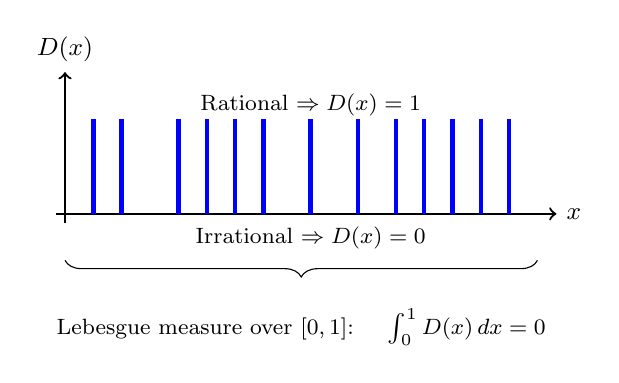
\begin{tikzpicture}[
    scale=1.2,
    every node/.style={font=\small},
    spike/.style={ultra thick, color=blue},
    axis/.style={->, thick},
    measure/.style={draw=none, fill=blue!10, opacity=0.4}
]

% Axes
\draw[axis] (-0.1,0) -- (5.2,0) node[right] {\( x \)};
\draw[axis] (0,-0.1) -- (0,1.5) node[above] {\( D(x) \)};

% Dots for rational spikes
\foreach \x in {0.3, 0.6, 1.2, 1.5, 1.8, 2.1, 2.6, 3.1, 3.5, 3.8, 4.1, 4.4, 4.7} {
    \draw[spike] (\x,0) -- (\x,1);
}

% Label on spike
\node at (2.6, 1.15) {\footnotesize Rational \( \Rightarrow D(x) = 1 \)};
\node at (2.6, -0.25) {\footnotesize Irrational \( \Rightarrow D(x) = 0 \)};

% Bracket (facing upward, placed lower below the axis)
\draw[decorate,decoration={brace,mirror,amplitude=6pt},yshift=-14pt]
  (0,0) -- (5,0);

% Text below bracket
\node at (2.5, -1.2) {\footnotesize Lebesgue measure over \([0,1]\): \quad \( \int_0^1 D(x)\, dx = 0 \)};

\end{tikzpicture}
\caption{Apparent patterns may be dense and tempting to interpret, but like the Dirichlet function, they can vanish under proper integration — exposing the illusion of structure.}
\end{figure}

This is the perfect analogy for false causation in high-frequency trading. Just like the Dirichlet function spikes at every rational, spurious correlations seem to occur constantly, but they vanish under rigorous integration via inclusion maps and measure theory. What appears to be a persistent signal is revealed to be noise: dense, but insignificant.

\begin{figure}[H]
\centering
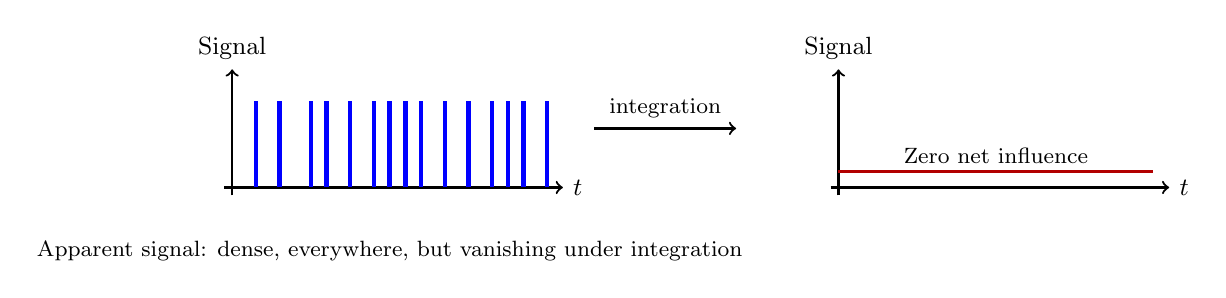
\begin{tikzpicture}[
    every node/.style={font=\small},
    spike/.style={ultra thick, color=blue},
    axis/.style={->, thick},
    smoothline/.style={very thick, red!70!black},
    measure/.style={draw=none, fill=blue!10, opacity=0.4}
]

% Shift left graph to the left
\begin{scope}[xshift=-1.5cm]
    % Axes left: raw signal
    \draw[axis] (-0.1,0) -- (4.2,0) node[right] {\( t \)};
    \draw[axis] (0,-0.1) -- (0,1.5) node[above] {Signal};

    % Spikes (false signals)
    \foreach \x in {0.3, 0.6, 1.0, 1.2, 1.5, 1.8, 2.0, 2.2, 2.4, 2.7, 3.0, 3.3, 3.5, 3.7, 4.0} {
        \draw[spike] (\x,0) -- (\x,1.1);
    }

    % Caption below left graph
    \node at (2, -0.8) {\footnotesize Apparent signal: dense, everywhere, but vanishing under integration};
\end{scope}

% Arrow to right side (integration lens)
\draw[->, thick] (3.1,0.75) -- (4.9,0.75) node[midway, above] {\footnotesize integration };

% Right graph: flat line (no signal survives)
\begin{scope}[xshift=6.2cm]
    \draw[axis] (-0.1,0) -- (4.2,0) node[right] {\( t \)};
    \draw[axis] (0,-0.1) -- (0,1.5) node[above] {Signal};

    % Flat result after integration
    \draw[smoothline] (0,0.2) -- (4,0.2);
    \node at (2, 0.4) {\footnotesize Zero net influence};
\end{scope}

\end{tikzpicture}
\caption{False causation in high-frequency data is like the Dirichlet function: spikes are dense but disappear under rigorous integration. What looks like signal is often just noise.}
\end{figure}


In this sense, Lebesgue integration acts as a filter --- not for smoothing out spikes, but for exposing which of them actually matter when viewed through the lens of a consistent probability measure. And more often than not, the spurious ones disappear.


\subsubsection{Concrete Example: Integration Over Reactive Trades}

\vspace{0.5em}
\noindent
Suppose you observe a sequence of rapid trades by a high-frequency strategy during a volatile macroeconomic event — say, a central bank rate announcement. The algorithm reacts quickly and often: short bursts of trades scattered through a millisecond-scale window. Every time you zoom in, there’s another spike of activity. It looks like the trading algorithm is “doing something.”

But when you apply a consistent measure — one that considers the total weight or contribution of these trades to the overall market — their impact washes out. They're reacting to the same event, not producing meaningful new information. The total measure assigned to these micro-responses is negligible.

\[
\mu(\text{reactive trades}) \approx 0.
\]

Lebesgue integration over these trades reveals this insignificance. Despite being dense in time, they have no weight — just like the Dirichlet function's spikes at the rationals.

\vspace{1em}
\begin{figure}[H]
\centering
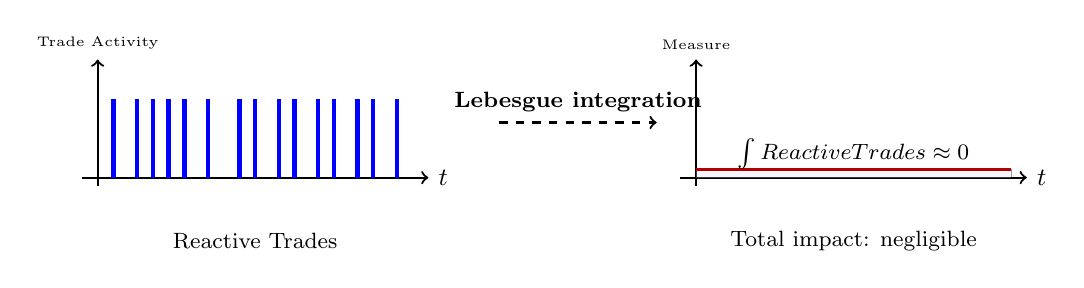
\begin{tikzpicture}[
    every node/.style={font=\small},
    axis/.style={->, thick},
    spike/.style={ultra thick, blue},
    integralarea/.style={fill=blue!10, opacity=0.4},
    dashedarrow/.style={->, thick, dashed},
    smoothline/.style={very thick, red!70!black}
]

% Left: set of reactive trades (dense spikes)
\begin{scope}[xshift=-1.8cm]
    \draw[axis] (-0.2,0) -- (4.2,0) node[right] {\( t \)};
    \draw[axis] (0,-0.1) -- (0,1.5) node[above] {\tiny Trade Activity};

    % Spikes (reactive trades)
    \foreach \x in {0.2, 0.5, 0.7, 0.9, 1.1, 1.4, 1.8, 2.0, 2.3, 2.5, 2.8, 3.0, 3.3, 3.5, 3.8} {
        \draw[spike] (\x,0) -- (\x,1);
    }

    % Label
    \node at (2, -0.8) {\footnotesize Reactive Trades};
\end{scope}

% Arrow indicating integration
\draw[dashedarrow] (3.3,0.7) -- (5.3,0.7) node[midway, above] {\footnotesize \textbf{Lebesgue integration}};

% Right: integrated result (area)
\begin{scope}[xshift=5.8cm]
    \draw[axis] (-0.2,0) -- (4.2,0) node[right] {\( t \)};
    \draw[axis] (0,-0.1) -- (0,1.5) node[above] {\tiny Measure};

    % Draw shaded area (tiny strip = ~0 measure)
    \draw[integralarea] (0,0) rectangle (4,0.1);
    \draw[smoothline] (0,0.1) -- (4,0.1);

    % Label
    \node at (2, 0.3) {\footnotesize \( \int \text{Reactive Trades} \approx 0 \)};
    \node at (2, -0.8) {\footnotesize Total impact: negligible};
\end{scope}

\end{tikzpicture}
\caption{Reactive trades during a macro event appear dense in time, but under integration their cumulative impact approaches zero — like measure-zero rational spikes.}
\end{figure}




\begin{figure}[H]
\centering
\begin{tikzpicture}[every node/.style={font=\footnotesize}]

% Panel 1 — Analyst is excited by the pattern
\comicpanel{0}{4}
  {Analyst A}
  {Analyst B}
  {Everywhere I look: a trade, a price twitch. I'm seeing structure! It's beautiful!}
  {(0,-0.6)}

% Panel 2 — Analyst B raises a math eyebrow
\comicpanel{6.5}{4}
  {Analyst A}
  {Analyst B}
  {Beautiful, yes. But have you tried integrating your discovery?}
  {(-0.2,-0.6)}

% Panel 3 — Analyst A hesitates
\comicpanel{0}{0}
  {Analyst A}
  {Analyst C}
  {Well... it looks a bit like the Dirichlet function. Spiky. Frequent. Very... rational.}
  {(0,0.5)}

% Panel 4 — Analyst C drops the measure-theoretic mic
\comicpanel{6.5}{0}
  {Analyst A}
  {Analyst C}
  {Exactly. Dense everywhere, measure zero. Integrate it — and poof, it’s gone.}
  {(0,0.6)}

\end{tikzpicture}
\caption{Some patterns are just Dirichlet functions in disguise — everywhere and worth nothing.}
\end{figure}






\subsection{Economic Impact of Ignoring Inclusion Maps}

\vspace{0.5em}
\noindent
Imagine a trading system made up of a thousand machines, each operating like an over-caffeinated intern on bad Wi-Fi. They're constantly scanning for signals --- trade bumps, price jitters, whatever seems to repeat --- and they act instantly, assuming causation where there may be none.

This is what happens when inclusion maps are ignored. The machines detect patterns that look like signals but are really statistical noise --- echoes of unrelated events or mutually triggered reactions to the same external cause. It’s like reading meaning into the spikes of the Dirichlet function: dense with activity, but empty when viewed through a proper lens.

Now let’s run the numbers.

\subsubsection{Case 1: Machines Trade on Spurious Correlations (No Inclusion Maps)}

\begin{itemize}
    \item Each machine executes 120 trades per second.
    \item The average loss per trade --- due to reacting to false signals --- is \$0.03.
    \item With 1,000 machines, this results in:

    \[
    120 \times 0.03 \times 1,000 = \text{\$3,600 lost per second}.
    \]
\end{itemize}

These machines aren't trading on insight: they’re chasing noise. And it costs them.

\subsubsection{Case 2: Machines Filter Out False Signals Using Inclusion Maps}

\begin{itemize}
    \item With inclusion maps in place, the machines ignore spurious correlations.
    \item Trades per machine drop to 90 per second: fewer, but smarter.
    \item The average profit per trade rises to \$0.08.
    \item With 1,000 machines, this becomes:

    \[
    90 \times 0.08 \times 1,000 = \text{\$7,200 earned per second}.
    \]
\end{itemize}

\textbf{Result:} By filtering out noise using inclusion maps — treating causality seriously rather than statistically — the system goes from losing \$3,600 every second to earning \$7,200. That’s a swing of \$10,800 per second, simply by shifting from reactive correlation to measured causation.

This isn’t just a philosophical point about math — it’s \$38.8 million per hour during market operations.


\begin{figure}[H]
\centering
\begin{tikzpicture}[every node/.style={font=\footnotesize}]

% Panel 1 — Frenzied trading bot
\comicpanel{0}{4}
  {Bot A}
  {Bot B}
  {I saw three bumps and a wiggle — deployed 120 trades per second. We're printing noise!}
  {(0,-0.6)}

% Panel 2 — Bot B checks the numbers
\comicpanel{6.5}{4}
  {Bot A}
  {Bot B}
  {You also lost \$3,600 per second. Congrats on outperforming entropy.}
  {(0,-0.5)}

% Panel 3 — Calm inclusion-mapped bot
\comicpanel{0}{0}
  {Bot C}
  {Bot D}
  {I filtered out spurious signals, traded less, and made \$7,200 per second.}
  {(0,0.6)}

% Panel 4 — Bot D delivers the verdict
\comicpanel{6.5}{0}
  {Bot A}
  {Bot D}
  {Turns out math isn't optional when money’s on the line.}
  {(0,0.6)}

\end{tikzpicture}
\caption{Inclusion maps: saving \$38.8 million an hour by not believing in trade wiggles.}
\end{figure}


\subsection{Final Takeaway: The Role of Mathematics in High-Frequency Trading}

\vspace{0.5em}
High-frequency trading operates in a world where milliseconds matter and patterns appear everywhere. But as we've seen, many of those patterns are like the Dirichlet function — dense, distracting, and ultimately meaningless when viewed through the right lens.

Without tools like inclusion maps, Lebesgue integration, and vector clocks:

\begin{itemize}
    \item We mistake coincidence for causation (acting on noise that just looks like signal).
    \item Our models chase false positives (reacting to patterns that vanish under proper integration).
    \item Entire trading systems amplify volatility, flooding the market with misguided decisions.
\end{itemize}

These mathematical tools form a kind of \textbf{epistemic firewall} — not just helping us model the market, but protecting us from ourselves. They give us a way to test whether a trade actually causes a price movement, or whether both are just reacting to the same macroeconomic tremor. They let us quantify how much we actually know, and whether that knowledge survives conditioning on reality.

\vspace{0.5em}
\noindent
\textbf{Bottom line:} Inclusion maps and vector clocks don’t just make our models cleaner; they make them safer. They ensure that our systems act on real signals, not illusions.

\begin{quote}
\textbf{Mathematics: the difference between chasing ghosts and capturing value; or between burning millions per second, and earning them.}
\end{quote}




\begin{figure}[H]
\centering
\begin{tikzpicture}[every node/.style={font=\footnotesize}]

% Panel 1 — Trader overwhelmed by patterns
\comicpanel{0}{4}
  {Trader A}
  {Trader B}
  {There are patterns everywhere! Look at all this market motion — it has to mean something.}
  {(0,-0.6)}

% Panel 2 — Trader B holds a book
\comicpanel{6.5}{4}
  {Trader A}
  {Trader B}
  {That's what the Dirichlet function said right before getting integrated into zero.}
  {(0,-0.5)}

% Panel 3 — Algorithm on fire
\comicpanel{0}{0}
  {Algo A}
  {Algo B}
  {Our model says BUY because of the third spike in the fifth harmonic. Also we’re on fire.}
  {(0,0.6)}

% Panel 4 — Calm analyst with math
\comicpanel{6.5}{0}
  {Algo A}
  {Analyst}
  {Inclusion maps. Vector clocks. Lebesgue. You know... the things that keep systems from hallucinating.}
  {(0,0.6)}

\end{tikzpicture}
\caption{Mathematics: the firewall between million-dollar models and million-dollar mistakes.}
\end{figure}
